\section{Experiment 4. 03.03.2020}\label{experiment-4.-03.03.2020}

It took place on 03.03.2020. The weather conditions were appropriate for experiment, although there was rain for a short time (approximately 10 minutes).

For the fourth trial, we implement sending of measurement messages only with \gls{http} protcol from \gls{ue} to \gls{command_n_center}. 

We aimed to find optimized positions for the \glspl{ue} in three cases (Sub-Optimal, Uniform, Near-Optimal).

We decided to reduce the area layout to 25x25 meters.

\glspl{ue} had initial coordinates shown in Table \ref{tab:exp4-initial-coordinates-ues}.

\begin{longtable}[]{@{}ll@{}}
	\caption{Initial coordinates for \glspl{ue}}\tabularnewline
	\toprule
	Unique ID & Coordinates\tabularnewline
	\midrule
	\endhead
	f072f812f48ce468 & (50.4056203, 10.5626057)\tabularnewline
	eb0b54819c69cf0c & (50.4056230, 10.5626126)\tabularnewline
	27349a2cde6592df & (50.4056445, 10.5625865)\tabularnewline
	51336504999bc1ca & (50.40567855, 10.5625238)\tabularnewline
	b1c225280d0ed13f & (50.4056924, 10.5624943)\tabularnewline
	\bottomrule
	\label{tab:exp4-initial-coordinates-ues}
\end{longtable}


The initial coordinates for \glspl{ap} are shown in Table \ref{tab:exp4-initial-coordinates-aps}.

\begin{longtable}[]{@{}ll@{}}
	\caption{Initial coordinates for \glspl{ap} }\tabularnewline
	\toprule
	AP & Coordinates\tabularnewline
	\midrule
	\endhead
	AP1 & (50.4056741, 10.5625129)\tabularnewline
	AP2 & (50.4056339, 10.5625975)\tabularnewline
	\bottomrule
	\label{tab:exp4-initial-coordinates-aps}
\end{longtable}

\subsection{Results}

The \gls{http} protocol helped to receive messages reliably, despite there was connection failures, we observed that the farther \gls{ue} is located from \gls{ap}, the less probable reception of the message. Retransmisson of messages implemented in \gls{gps_android} partly mitigated losses.

We found out that network speed measurements were not significant, because there was markedly seen difference between \texttt{uplink} and \texttt{downlink} speed, uplink tests threw timeout exception in case of larger distance between a \gls{ue} and a \gls{access_point}, because the communication took longer and the session finished.

The experiment is divided into four parts:

\begin{itemize}
\tightlist
\item
  Before 11:05 - Sub-Optimal case
\item
  11:05 - 11:08 - Uniform case
\item
  11:08 - 11:12 - Near-Optimal case
\item
  11:12 - 11:15 Sub-Optimal to compare to the suggested positions
\end{itemize}

\subsubsection{Sub-Optimal case}

The first case is the most profitable from the signal quality point of
view. The \glspl{ap} are implicitly located at the same distance from the
connected \glspl{ue}. Signal changes can be seen in Figure \ref{fig:signal-quality-changes-sub-optimal} - despite this case is expected to have the best link parameters, \acrshort{rss} is unstable for \glspl{ue}, possible reason for this - differences in phone generations, e.g. modern phones also include more advanced \gls{wifi} model.

\begin{figure}[H]
	\centering
	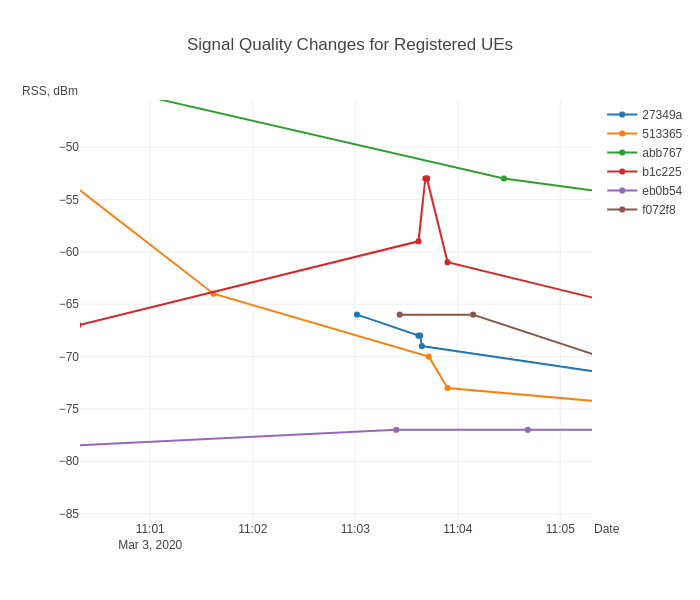
\includegraphics[width=0.7\linewidth,keepaspectratio]{images/Exp4_Suboptimal.png}
\caption{Signal Quality changes in Sub-Optimal case}
\label{fig:signal-quality-changes-sub-optimal}
\end{figure}

Despite the \glspl{ap} were located close to \glspl{ue}, the \acrshort{rss} level varies noticeably. However, only in this case the speed and signal quality measurement were the most stable among all cases.

\subsubsection{Uniform case}

In this case, the \glspl{ap} are located with equal distance from the \gls{command_n_center}.

\begin{figure}[H]
	\centering
	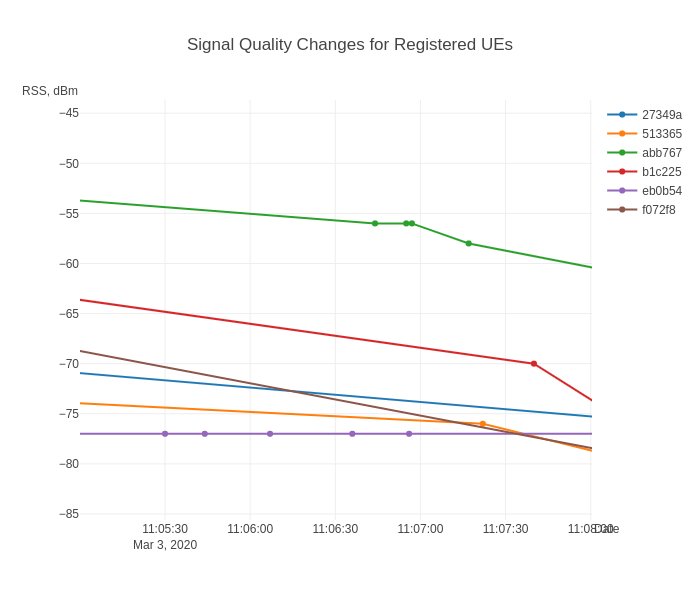
\includegraphics[width=0.7\linewidth,keepaspectratio]{images/Exp4_Uniform.png}
\caption{Signal Quality changes in Uniform case}
\label{fig:signal-quality-changes-uniform-optimal}
\end{figure}

Figure \ref{fig:signal-quality-changes-uniform-optimal} depict \acrshort{rss} changes in Uniform case. Link measurement are more steady and keep on the same level for the majority of \gls{ue}, however we encountered speed test failed.

\subsubsection{Near-optimal case}

The third case simulates the situation where the \glspl{ap} are placed
uniformly far from centers of \glspl{ue} clusters.

Figure \ref{fig:signal-quality-changes-near-optimal} demostrates that measured \acrshort{rss} lower than in Uniform case because of larger distance between \glspl{ap} and \glspl{ue} approximately on 10-15 dBm.

\begin{figure}[H]
	\centering
	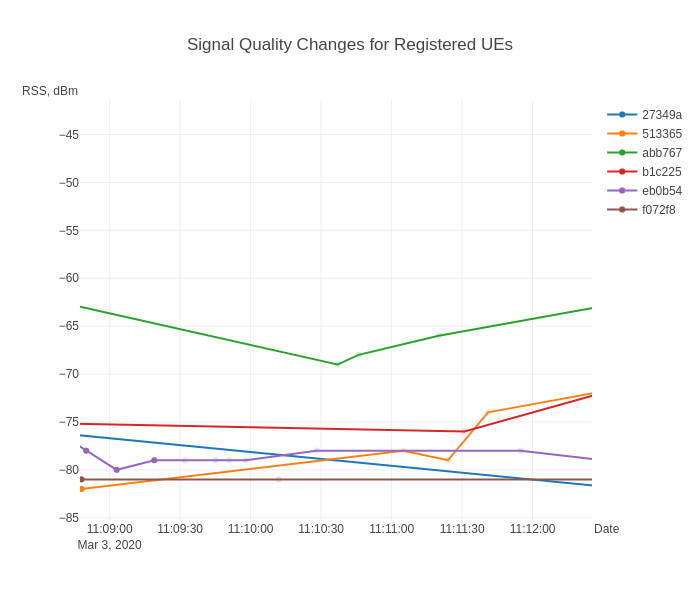
\includegraphics[width=0.7\linewidth,keepaspectratio]{images/Exp4_Near_Optimal.png}
\caption{Signal Quality changes in Near-optimal case}
\label{fig:signal-quality-changes-near-optimal}
\end{figure}

\subsubsection{Comparison between Sub-Optimal case, and the suggested
positions}

To check the validity of \glspl{uav} layout optimization algorithm, we place the \glspl{ap} in a Sub-Optimal case position. Figure \ref{fig:ues-positions-for-optimization} represents the most recent positions  of \glspl{ue} as input data used for optimization tasks.

\begin{figure}[H]
	\centering
	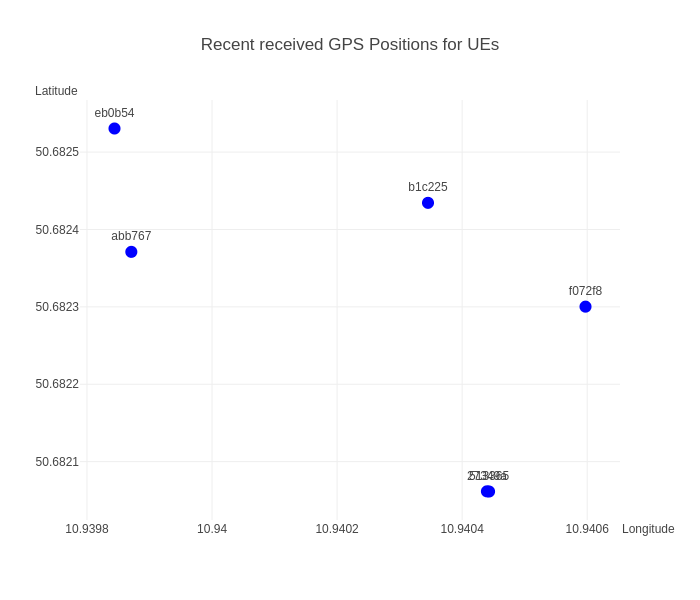
\includegraphics[width=0.5\linewidth,keepaspectratio]{images/Exp4_UEs_Location_to_optimize.png}
\caption{The \glspl{ue} coordinates used to optimize \glspl{uav} positions}
\label{fig:ues-positions-for-optimization}
\end{figure}

The coordinates for \textbf{27349a2cde6592df} and
\textbf{51336504999bc1ca} overlap.

The most recent received coordinates for \glspl{ue} used to schedule an optimization task with the following parameters:

\begin{itemize}
\tightlist
\item
  Number of clusters: 2
\item
  Estimation method: ``clustering''
\end{itemize}

The ``simplex'' method against two clusters is not possible. Instead we use 'clustering' method which uses K-means clusterization algorithm. Figure \ref{fig:ues-positions-and-suggested-optimal-positions-for-uavs} demonstrate positions for \glspl{ue} as blue dots and suggested coordinates for two \glspl{uav} as black box.

\begin{figure}[H]
	\centering
	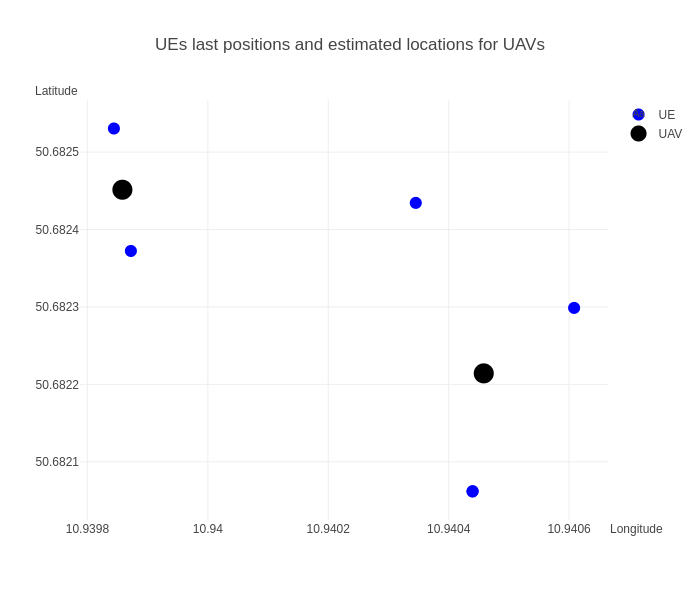
\includegraphics[width=0.5\linewidth,keepaspectratio]{images/Expt4_Estimated UAVs_locations.png}
\caption{Result of optimization task to obtain optimal positions for \glspl{uav}}
\label{fig:ues-positions-and-suggested-optimal-positions-for-uavs}
\end{figure}

The suggested optimal coordinates for \glspl{ap} are shown in Table \ref{tab:optimal-coordinates}.

\begin{longtable}[]{@{}lll@{}}
\caption{Suggested optimal positions for \glspl{uav} }\tabularnewline
\toprule
AP & Real coordinates & Suggested coordinates\tabularnewline
\midrule
\endhead
AP1 & (50.4056741, 10.5625129) & (50.68221, 10.94046)\tabularnewline
AP2 & (50.4056339, 10.5625975) & (50.68245, 10.93986)\tabularnewline
\bottomrule
\label{tab:optimal-coordinates}
\end{longtable}

Figure \ref{fig:optimized-coordinates-on-logical-map} shows on the map real and suggested optimal coordinates for \gls{uav}. Clearly seen these new positions can drop out connected clients because of large distance. Figure \ref{fig:optimized-coordinates-satellite-map} depict these coordinates on the map from satellite point of view.

\begin{figure}[H]
	\centering
	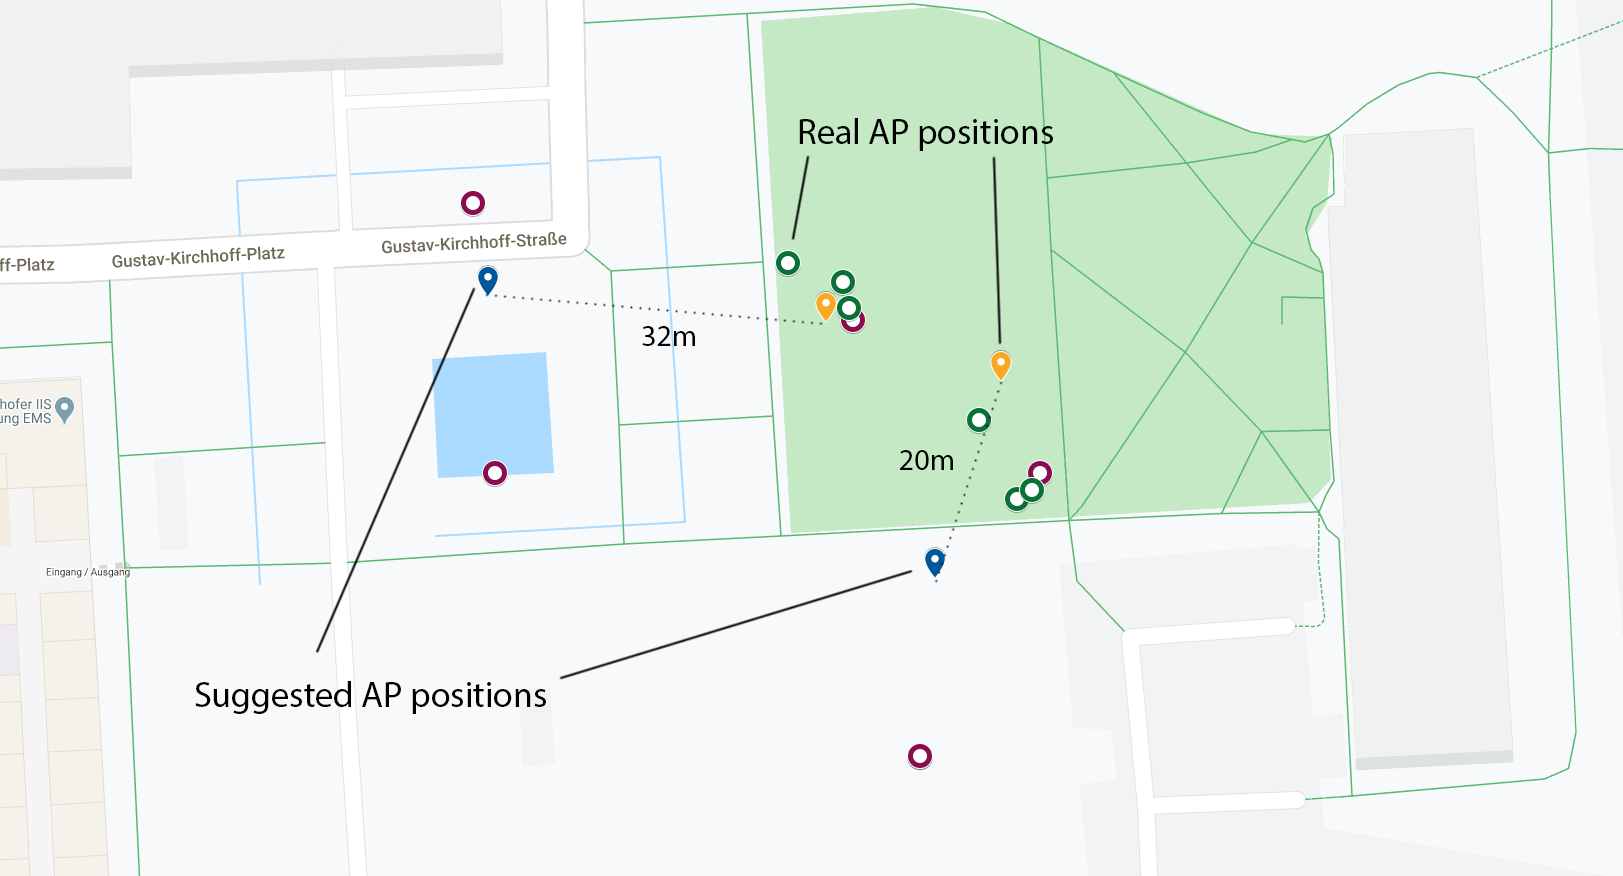
\includegraphics[width=\linewidth,keepaspectratio]{images/Expt4_Result_of_optimization_map_with_names.png}
\caption{Original and Optimized Coordinates: A map with tags.}
\label{fig:optimized-coordinates-on-logical-map}
\end{figure}

\begin{figure}[H]
	\centering
	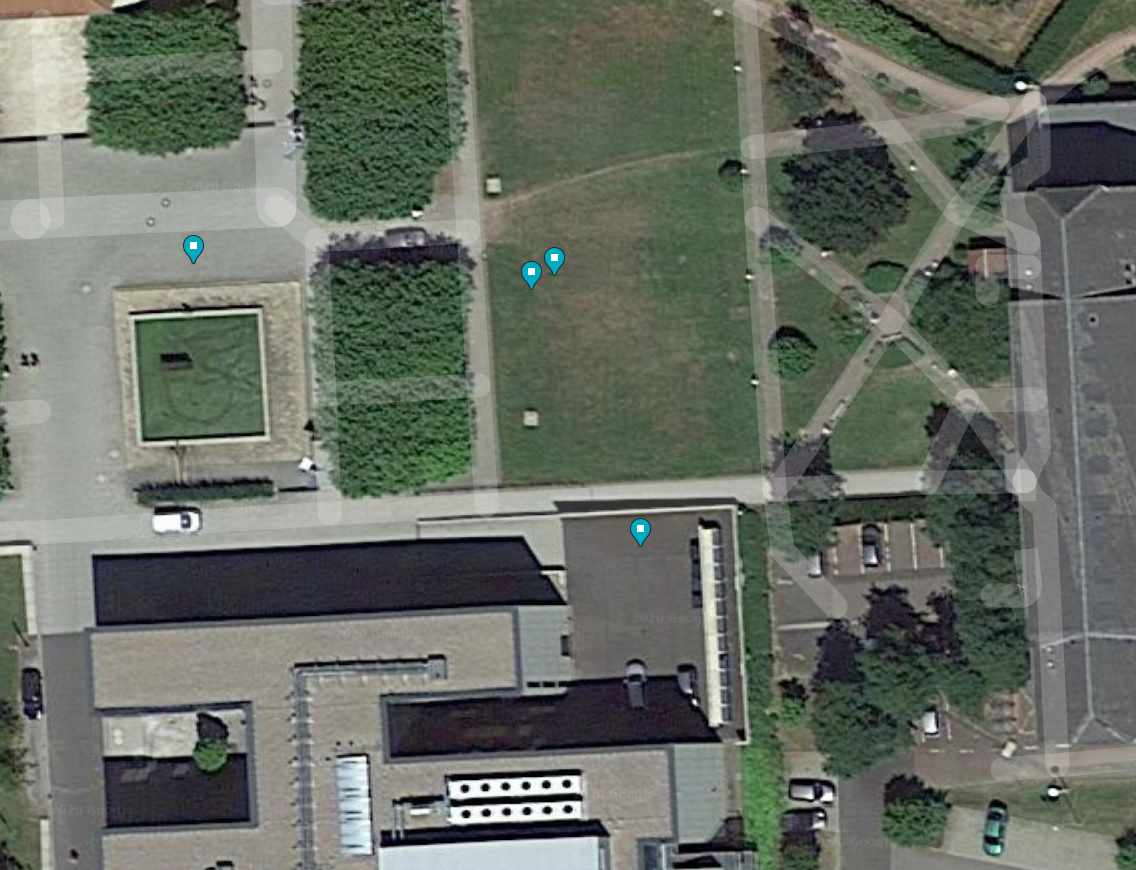
\includegraphics[width=\linewidth,keepaspectratio]{images/Expt4_Result_of_optimization_sattelite.png}
\caption{Original and Optimized Coordinates for \glspl{uav}: A picture from satellite}
\label{fig:optimized-coordinates-satellite-map}
\end{figure}

``Clustering'' algorithm performs simple K-means cluster calculation
based on \gls{gnss} coordinates for \glspl{ue}. The result provides insights about that layout optimization algorithms relying solely on the coordinate input data can result in a biased solution.

\subsection{Outcome}

Finally, we have managed to test the framework and estimate an optimized position for \glspl{uav} which were represented by \gls{wifi} access points. The results showed that the framework match requirements, however should be redesigned and evaluated on updated data.
